\documentclass[thesis.tex]{subfiles}

\begin{document}
    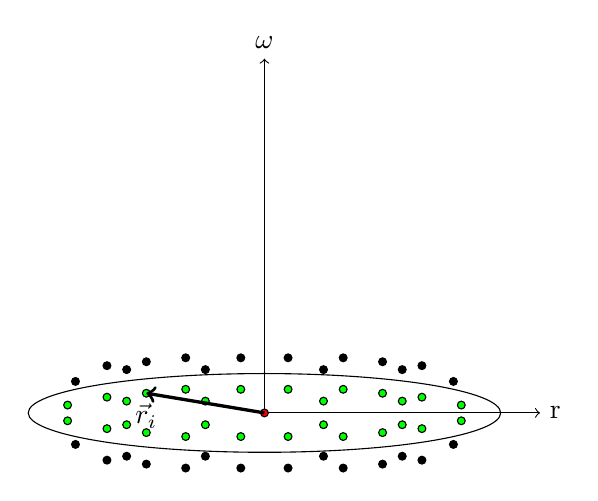
\begin{tikzpicture}[domain=-3:3]
        % оси
        \draw[->] (0,0) -- (0,4.5) node[at end,above] {$\omega$};
        \draw[->] (0,0) -- (3.5,0) node[at end, right] {r};

        % область сглаживания
        \draw (0,0) ellipse (3 and 0.5);

        % ядро сглаживания
        \draw[color=black, thick] plot function{9*(exp(-x*x/15.0)-exp(-3*3/15.0))};

        % интегрируемая частица
        \node[draw,circle,inner sep=1pt,fill=red] at (0,0) {};

        % частицы внутри области
        \node[draw,circle,inner sep=1pt,fill=green] at (1   ,0.3) {};
        \node[draw,circle,inner sep=1pt,fill=green] at (2.5 ,0.1) {};
        \node[draw,circle,inner sep=1pt,fill=green] at (2.0 ,0.2) {};
        \node[draw,circle,inner sep=1pt,fill=green] at (1.5 ,0.25) {};
        \node[draw,circle,inner sep=1pt,fill=green] at (1.75,0.15) {};
        \node[draw,circle,inner sep=1pt,fill=green] at (0.75,0.15) {};
        \node[draw,circle,inner sep=1pt,fill=green] at (0.3 ,0.3) {};

        \node[draw,circle,inner sep=1pt,fill=green] at (-1   ,0.3) {};
        \node[draw,circle,inner sep=1pt,fill=green] at (-2.5 ,0.1) {};
        \node[draw,circle,inner sep=1pt,fill=green] at (-2.0 ,0.2) {};
        \node[draw,circle,inner sep=1pt,fill=green] at (-1.5 ,0.25) {};
        \node[draw,circle,inner sep=1pt,fill=green] at (-1.75,0.15) {};
        \node[draw,circle,inner sep=1pt,fill=green] at (-0.75,0.15) {};
        \node[draw,circle,inner sep=1pt,fill=green] at (-0.3 ,0.3) {};

        \node[draw,circle,inner sep=1pt,fill=green] at (1   ,-0.3) {};
        \node[draw,circle,inner sep=1pt,fill=green] at (2.5 ,-0.1) {};
        \node[draw,circle,inner sep=1pt,fill=green] at (2.0 ,-0.2) {};
        \node[draw,circle,inner sep=1pt,fill=green] at (1.5 ,-0.25) {};
        \node[draw,circle,inner sep=1pt,fill=green] at (1.75,-0.15) {};
        \node[draw,circle,inner sep=1pt,fill=green] at (0.75,-0.15) {};
        \node[draw,circle,inner sep=1pt,fill=green] at (0.3 ,-0.3) {};

        \node[draw,circle,inner sep=1pt,fill=green] at (-1   ,-0.3) {};
        \node[draw,circle,inner sep=1pt,fill=green] at (-2.5 ,-0.1) {};
        \node[draw,circle,inner sep=1pt,fill=green] at (-2.0 ,-0.2) {};
        \node[draw,circle,inner sep=1pt,fill=green] at (-1.5 ,-0.25) {};
        \node[draw,circle,inner sep=1pt,fill=green] at (-1.75,-0.15) {};
        \node[draw,circle,inner sep=1pt,fill=green] at (-0.75,-0.15) {};
        \node[draw,circle,inner sep=1pt,fill=green] at (-0.3 ,-0.3) {};

        % частицы вне области
        \node[draw,circle,inner sep=1pt,fill] at (2.4 ,0.4) {};
        \node[draw,circle,inner sep=1pt,fill] at (1   ,0.7) {};
        \node[draw,circle,inner sep=1pt,fill] at (2.0 ,0.6) {};
        \node[draw,circle,inner sep=1pt,fill] at (1.5 ,0.65) {};
        \node[draw,circle,inner sep=1pt,fill] at (1.75,0.55) {};
        \node[draw,circle,inner sep=1pt,fill] at (0.75,0.55) {};
        \node[draw,circle,inner sep=1pt,fill] at (0.3 ,0.7) {};

        \node[draw,circle,inner sep=1pt,fill] at (-2.4 ,0.4) {};
        \node[draw,circle,inner sep=1pt,fill] at (-1   ,0.7) {};
        \node[draw,circle,inner sep=1pt,fill] at (-2.0 ,0.6) {};
        \node[draw,circle,inner sep=1pt,fill] at (-1.5 ,0.65) {};
        \node[draw,circle,inner sep=1pt,fill] at (-1.75,0.55) {};
        \node[draw,circle,inner sep=1pt,fill] at (-0.75,0.55) {};
        \node[draw,circle,inner sep=1pt,fill] at (-0.3 ,0.7) {};

        \node[draw,circle,inner sep=1pt,fill] at (2.4 ,-0.4) {};
        \node[draw,circle,inner sep=1pt,fill] at (1   ,-0.7) {};
        \node[draw,circle,inner sep=1pt,fill] at (2.0 ,-0.6) {};
        \node[draw,circle,inner sep=1pt,fill] at (1.5 ,-0.65) {};
        \node[draw,circle,inner sep=1pt,fill] at (1.75,-0.55) {};
        \node[draw,circle,inner sep=1pt,fill] at (0.75,-0.55) {};
        \node[draw,circle,inner sep=1pt,fill] at (0.3 ,-0.7) {};

        \node[draw,circle,inner sep=1pt,fill] at (-2.4 ,-0.4) {};
        \node[draw,circle,inner sep=1pt,fill] at (-1   ,-0.7) {};
        \node[draw,circle,inner sep=1pt,fill] at (-2.0 ,-0.6) {};
        \node[draw,circle,inner sep=1pt,fill] at (-1.5 ,-0.65) {};
        \node[draw,circle,inner sep=1pt,fill] at (-1.75,-0.55) {};
        \node[draw,circle,inner sep=1pt,fill] at (-0.75,-0.55) {};
        \node[draw,circle,inner sep=1pt,fill] at (-0.3 ,-0.7) {};

        % радиус вектор
        \draw[->,very thick] (0,0) -- (-1.5 ,0.25) {} node[at end, below] {${\vec r}_i$};

    \end{tikzpicture}
\end{document}
